\section{Samostatná práce člena týmu\ --\ Ondřej Fojt}
\label{sec:individual_work_ondra}

\subsection{Výběr tématu, popis provedeného průzkumu s uživatelem, analýza uživatelských potřeb a klíčových problémů, navržená sada změn}

\subsubsection*{Výběr tématu}

{\large Můj návrh:}

Checklist/TODO manažer na hlídání deadline pro kohokoliv, kdo dělá více projektů zároveň.


{\noindent \large Vybraný návrh v týmu:}

Medicínský systém pro přihlašování klientů na procedury/sezení/vyšetření. Zaměření především na přihlašování klientů a zobrazení těchto přihlášek

\subsubsection*{Provedený průzkum}

{ \noindent \large Technická podpora zubní ordinace:}

U přihlašování pacient sám neví na jak dlouhou dobu se má objednat. Většinou pacienti spíše volají/píší emaily, protože si nejsou jistý jak se objednat. Objednat se by mělo zabrat co nejméně kroků

{\noindent \large Pacient co se chce přihlásit:}

I když je tlačítko pro odeslání/pokračování velké a má velký kontrast pokud je umístěno úplně ve spodku obrazovky, tak si ho dost lidí nemusí rychle všimnout. V naléhavém případě může být online přihlašování restriktivní (když někoho bolí zub, tak asi nebude chtít čekat 2 týdny)

{\noindent \large Doktor provádějící vstupní prohlídky}

Dětské rehabilitační oddělení
\begin{itemize}
    \item  K lékařům na prohlídku se neobjednává. Je důležité, aby si lékaři mohli na pacienty vyčlenit čas, co nejdříve. Mají frontu, kde pacienti případně počkají. Náhled do fronty vidí doktoři i skrze informační systém nemocnice, kde mohou vidět některé zprávy o pacientech, číslo pojišťovny, zaměstnavatele atp. Lékaři dávají i termíny, kdy mají přijít na kontrolu bez nutnosti registrace.
    \item  V ošetřovně je jeden telefon, který berou doktoři. Přesto, že se neobjednává, tak 20\% lidí zavolá, aby se ujistili či objednali. Případy, které lze odložit se snaží doktoři přesunout na místa, kdy chodí málo lidí. 
    \item  Na jednotlivé rehabilitační procedury lékaři pevně objednávají pacienty v rozmezí ambulantní doby. Oddělení poskytuje různé služby jako jsou např. laser, magnet a fyziocvičení. 
    \item  Doktoři mají kalendář do kterého si dělají čárky, které znázorňují obsazenost procedur. Čárka značí pacienta. Do objednávkových sešitů se zaznamená jméno a kontakt v případě nemoci doktora. V takovém případě se každému zavolá a přesune se ho. Každá procedura má svojí obsazenost. Např. je dobré aby magnet byl značně obsazený, když už je zapnutý, ale aby i bylo možné na poslední chvíli někoho přidat. Magnet má doporučenou obsazenost 90\%.
    \item  Nevýhodou je, že již není k dispozici procentuální obsazenost, že si nelze lehce vyhledat termíny pacienta. Nelze zjistit z domova, zda mám dnes volněji. Je třeba zadat údaje dvakrát - do kalendáře a do papírku potvrzující objednání. Nelze zjistit z domova, zda mám dnes volněji. 
    \item  Výhodou systému je zažitost a netěžká obsluha. Netřeba zapínat tablet či počítač.
    \item  Potřeby uživatele, lékařů a fyzioterapeutů, jsou evidovat pacienty a případně je zarezervovat, znát volné termíny, možnost zkontrolovat, kdo přijde. Je potřeba evidovat čísla pro pojišťovnu pro vyplacení peněz.
\end{itemize}

\subsubsection*{Analýza potřeb a klíčových problémů}

U některých registrací není dopředu známý čas. Mnoho lékařů používá pouhé kalendáře (online nebo papírové) -> jakou motivaci mají k používání našeho systému? Přihlašování akutních/speciálních případů v rozumném čase.

První vyšetření u lékaře se nedá vě většině případů naplánovat. Doktorovi se hodí vidět zaplněnost jednotlivých služeb, aby se mohl rozhodnout kam pacienta objedná, pokud může být rehabilitován více různými procedurami.
Fyzioterapeutovi by se spíše hodilo vidět jména a kontakty pacientů v rámci registrací a aby je mohli sami registrovat na termín, který není příliš zaplněný.


\subsubsection*{Navržená sada změn}
\noindent\emph{Návrh I.}

Pacient by měl možnost vybrat více termínů, které se mu hodí a po určité době mu bude sděleno, kdy má přijít.

\noindent\emph{Návrh II.}

Pro akutní případy umožnit zkrácení délky okna termínu, aby měli možnost přijít co možná nejdříve.

\noindent\emph{Návrh III.}

Při výběru v rámci přihlašovacího formuláře rovnou zobrazit další krok místo nutnosti klikat na tlačítko další.

%\newpage
\subsection{Popis současného řešení\ --\ jaké nástroje uživatel používá, \\
popř. obrázky/screenshoty současného řešení/reálné situace}

\noindent\emph{Poznámky v kalendáři/online dokumentu/e-mailech} 
\begin{itemize}
    \item[+] Není potřeba získat a naučit se nový systém
    \item[--] Nestrukturované
    \item[--] náročné na vyhledávání určitých přihlášek
    \item[--] potřebná komunikace pro přihlášení ze strany zaměstnance
\end{itemize}

\noindent\emph{XDENT viz \ref{fig:Ondra_xdent_admin}.}
\begin{itemize}
    \item[+] Umožňuje online přihlašování, chat s pacientem, upomínky...
    \item[+/--] Specializováno pro zubní ordinace
    \item[--] Měsíční poplatky za licenci a služby 
\end{itemize}

\begin{figure}[htbp]
    \centering
    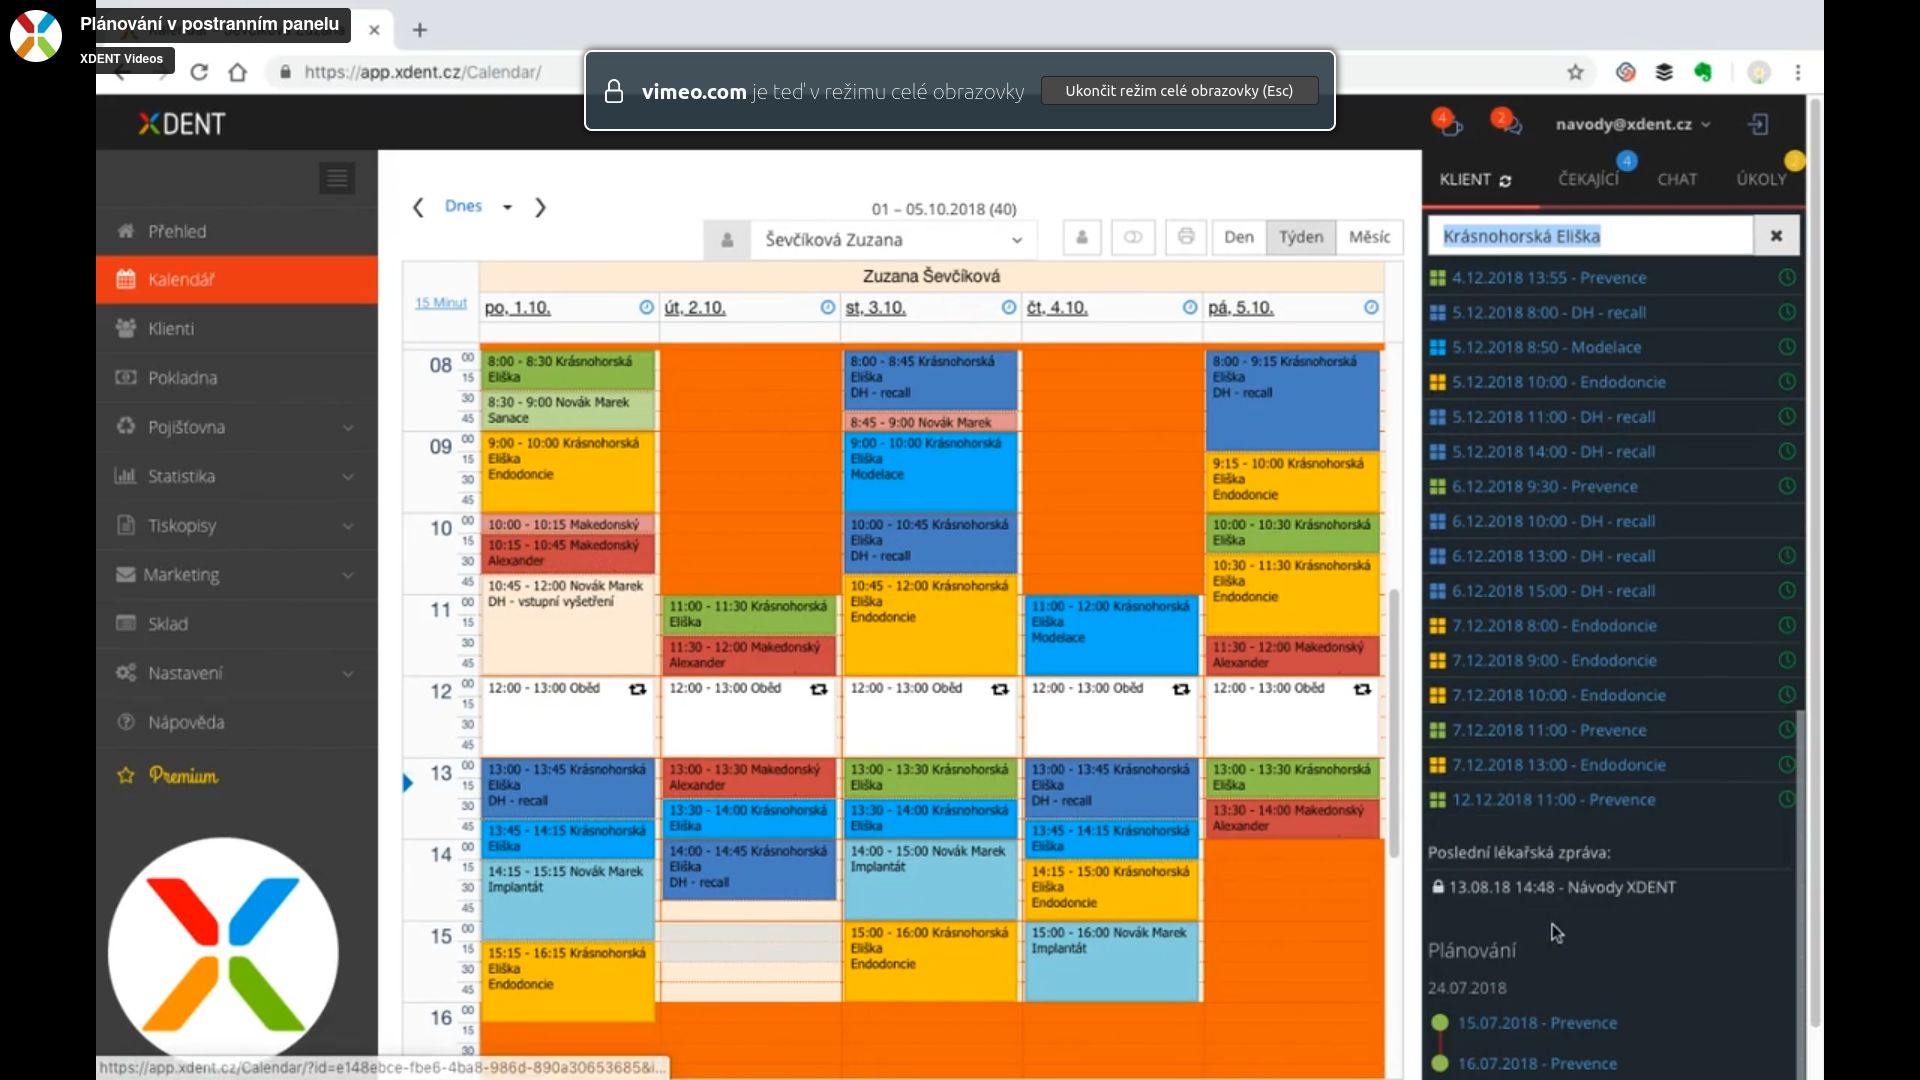
\includegraphics[width = \textwidth]{doc/latex/fig/ondra/xdent-admin.png}
    \caption{XDENT: Pohled přihlášeného zaměstnance/administrátora}
    \label{fig:Ondra_xdent_admin}
\end{figure}

\newpage

\noindent\emph{Týmuj}
\begin{itemize}
    \item[+] Každý přihlášený může uvést k dané událost, zda se zúčastní nebo ne
    \item[--] není přímo z lékařství -> vytvářet termíny může každý
\end{itemize}

\subsection{Návrh uživatelského rozhraní, makety rozhraní, testování pomocí maket rozhraní}

\emph{Část projektu v týmu: Návrh rozhraní pro zaměstnance}

\subsubsection*{Návrh}

\begin{itemize}
    \item Lze najít nejbližší události
    \item Lze Zobrazit události ostatních zaměstnanců
    \item Jednoduché zobrazení podrobností o události
    \item Přidání/změny událostí pouze po potvrzení interakcí
    \item Zaměstnanec(dle vnitřní politiky) může vyhledávat/měnit časy, kdy může poskytovat jednotlivé služby
\end{itemize}

\subsubsection*{Maketa}

{\noindent\Large Popis makety}

Hlavní stránka viz \ref{fig:Ondra_figma_mainpage} slouží pro rychlé zorientování v nadcházejících\\ událostech pro daného zaměstnance. 
Umožňuje změnit pohled, což znamená ukázat události, rozvrh, jiného zaměstnance. Tohle se může hodit například pokud potřebuji vědět, kde ve který čas někoho můžu najít.
Dále se na stránce nachází seznam několika nejbližších tedy nadcházejících událostí. Zobrazují se zde služby, které zaměstnanec poskytuje a také vnitřní organizační záležitosti firmy/organizace.
Na spodní straně stránky se nachází kalendář událostí, pro lepší orientaci v termínech událostí. V něm lze vyhledávat, tisknout ho a v případě nutnosti také upravovat.
Úprava událostí by měla být možná pouze daným zaměstnancem nebo jeho nadřízenými.

Vyskakovací okno ukázané na obrázku \ref{fig:Ondra_figma_event_detail} se zobrazí po kliknutí na událost.
Okno obsahuje název události, datum a čas, místo konání, zodpovědnou osobu(v případě služeb bude obsahovat jméno zaměstnance 
na jehož pohled se například díváme, ale nemusí tomu tak vždy být), jednotlivé účastníky, u kterých bude možnost otevřít okno s kontaktem na danou osobu, 
a nakonec popis události, který dle události může vyplňovat zaměstnanec nebo klient, který se na událost přihlásil.
Ve vyskakovacím okně nelze nic měnit pokud není zapnutý režim pro úpravu událostí.

Protože každý zaměstnanec může poskytovat různé služby a také se můžou dramaticky 
lišit pracovní doby zaměstnanců je k dispozici stránka pro správu nabízených služeb viz obr. \ref{fig:Ondra_figma_services}.
Stejně jako u událostí je zde možnost ukázat služby ostatních zaměstnanců a stejně tak úprava údajů v rámci poskytovaných služeb.
Samotné služby představuje sada rozbalovacích oken, ve kterých se nachází týdenní rozpis časů, mezi nimiž se lze u daného zaměstnance přihlásit na tuto službu.
V rámci nabídek služeb lze rychle vidět, které služby zaměstnanec neposkytuje. 

Na maketu se lze podívat v read-only odkazu \href{https://www.figma.com/file/h0A4BXg6jb5XL084kGsEIn/ITU---Registra%C4%8Dn%C3%AD-syst%C3%A9m-pro-rehabilita%C4%8Dn%C3%AD-slu%C5%BEby?node-id=64%3A288}{zde.}
Není nějak vysoce propracovaná, ale přechody fungují.

\begin{figure}[htbp]
    \centering
    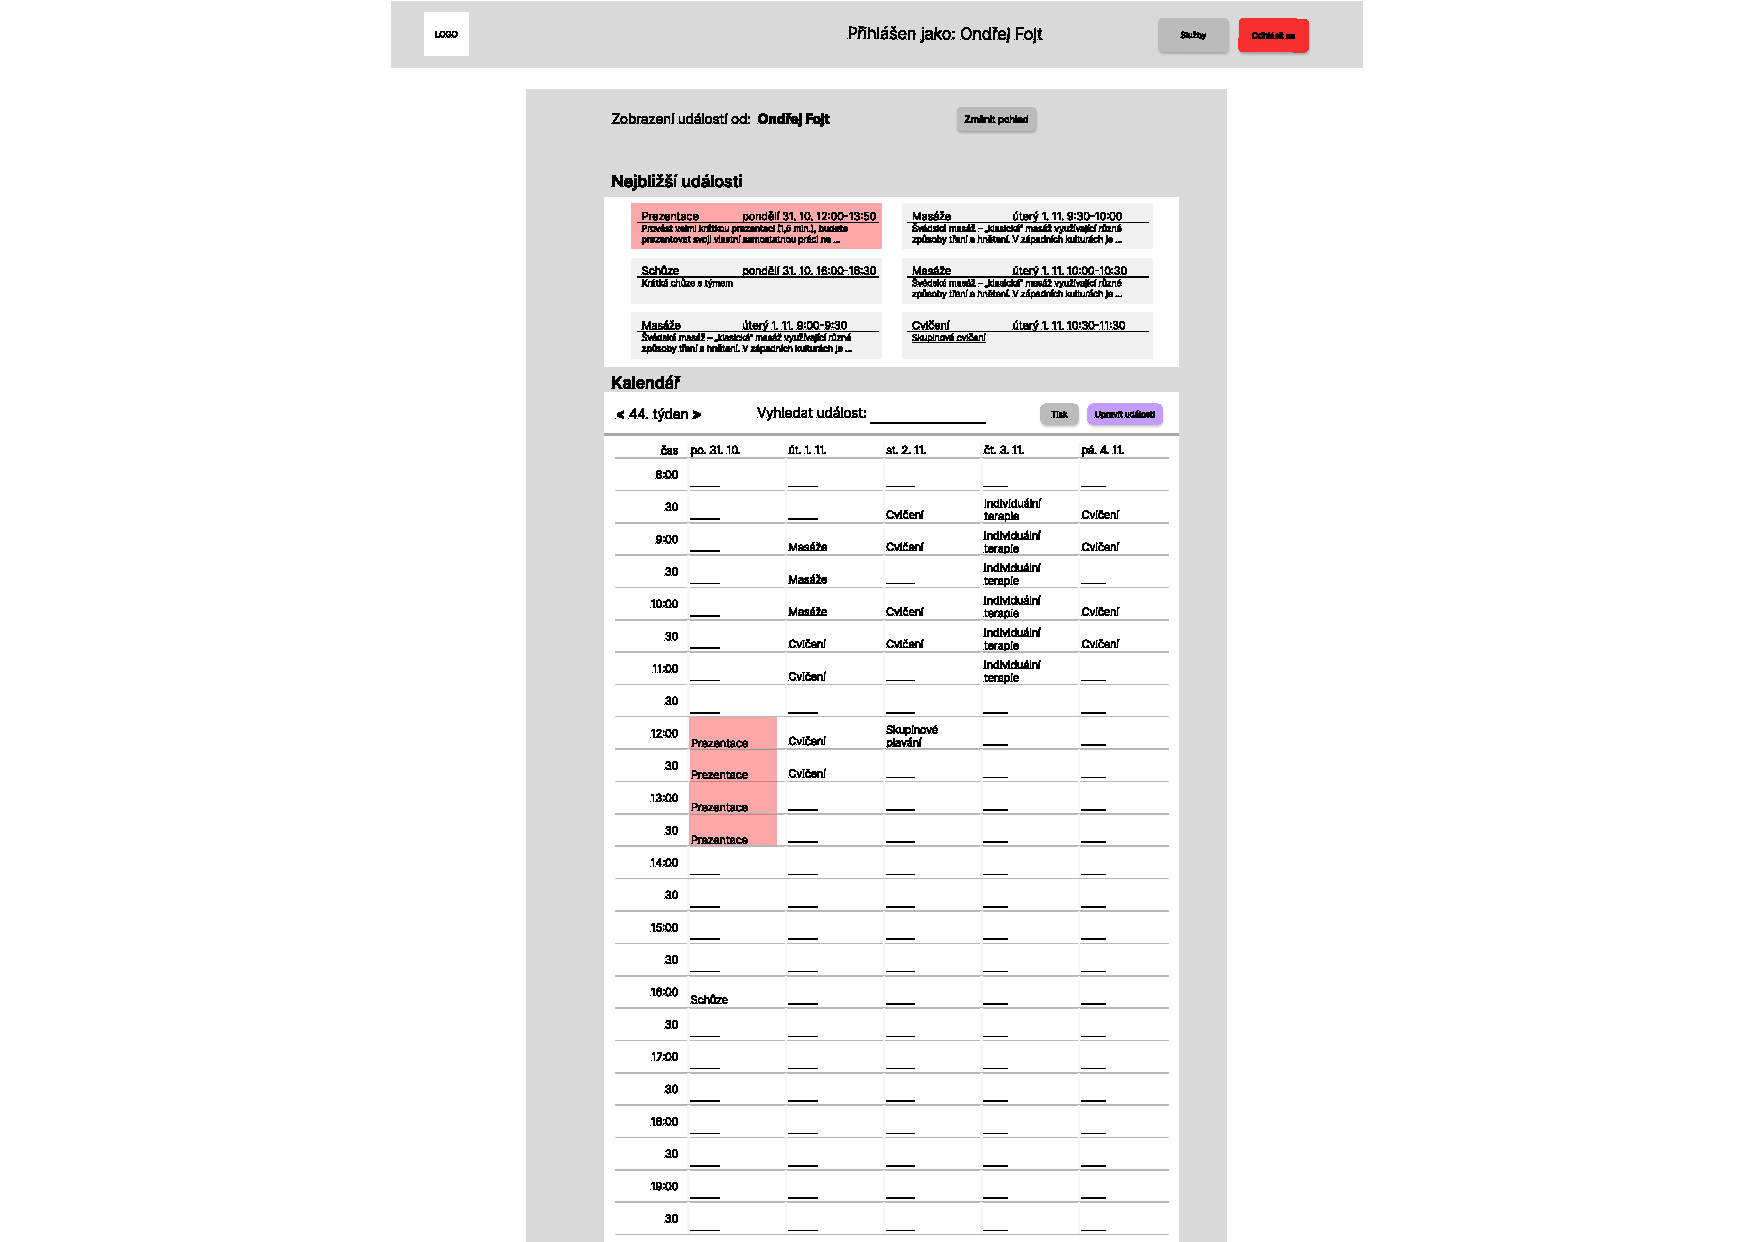
\includegraphics[width = \textwidth, trim=200 300 200 0, clip]{doc/latex/fig/ondra/figma1.pdf}
    \caption{Hlavní strana s výpisem nejbližších událostí a kalendářem událostí}
    \label{fig:Ondra_figma_mainpage}
\end{figure}

\begin{figure}[htbp]
    \centering
    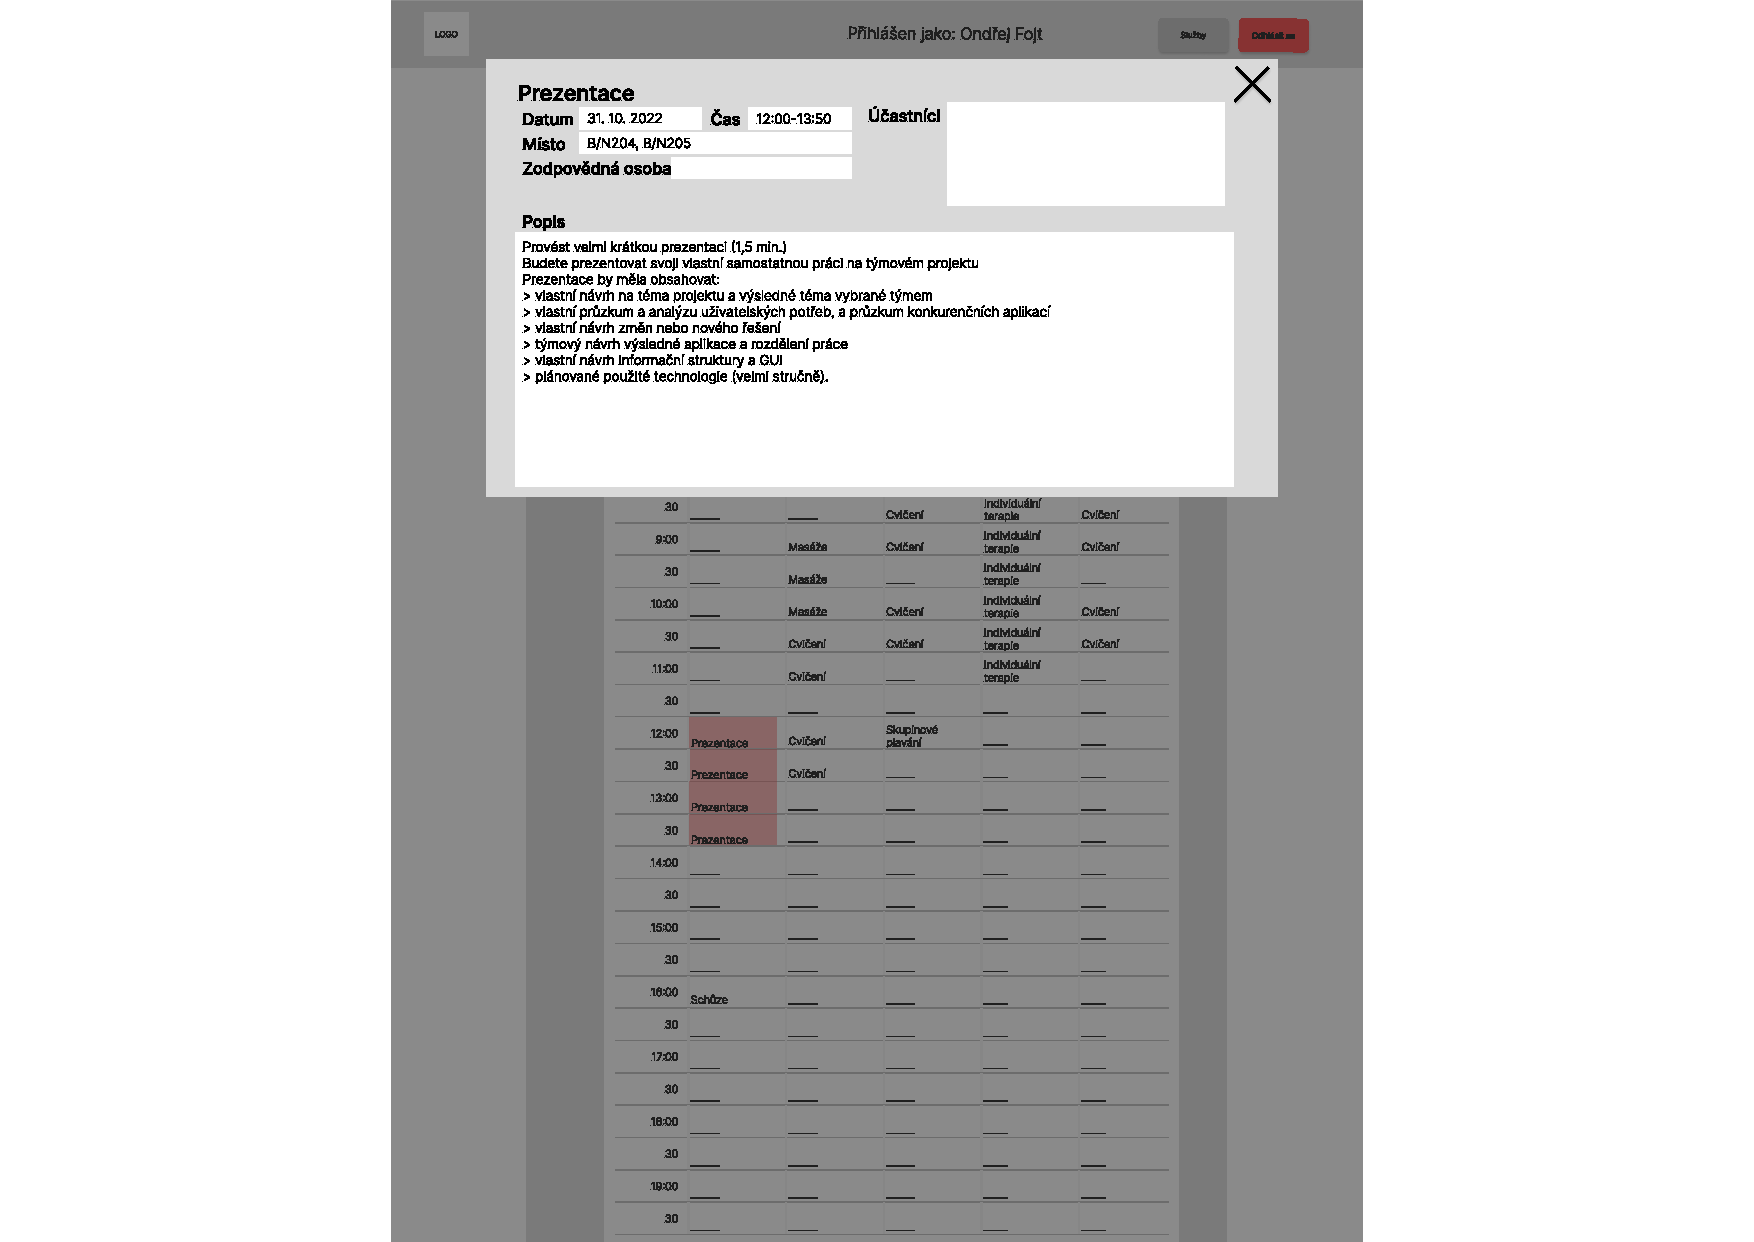
\includegraphics[width = \textwidth, trim=200 380 200 0, clip]{doc/latex/fig/ondra/figma2.pdf}
    \caption{Zobrazení údajů o události}
    \label{fig:Ondra_figma_event_detail}
\end{figure}

\begin{figure}[htbp]
    \centering
    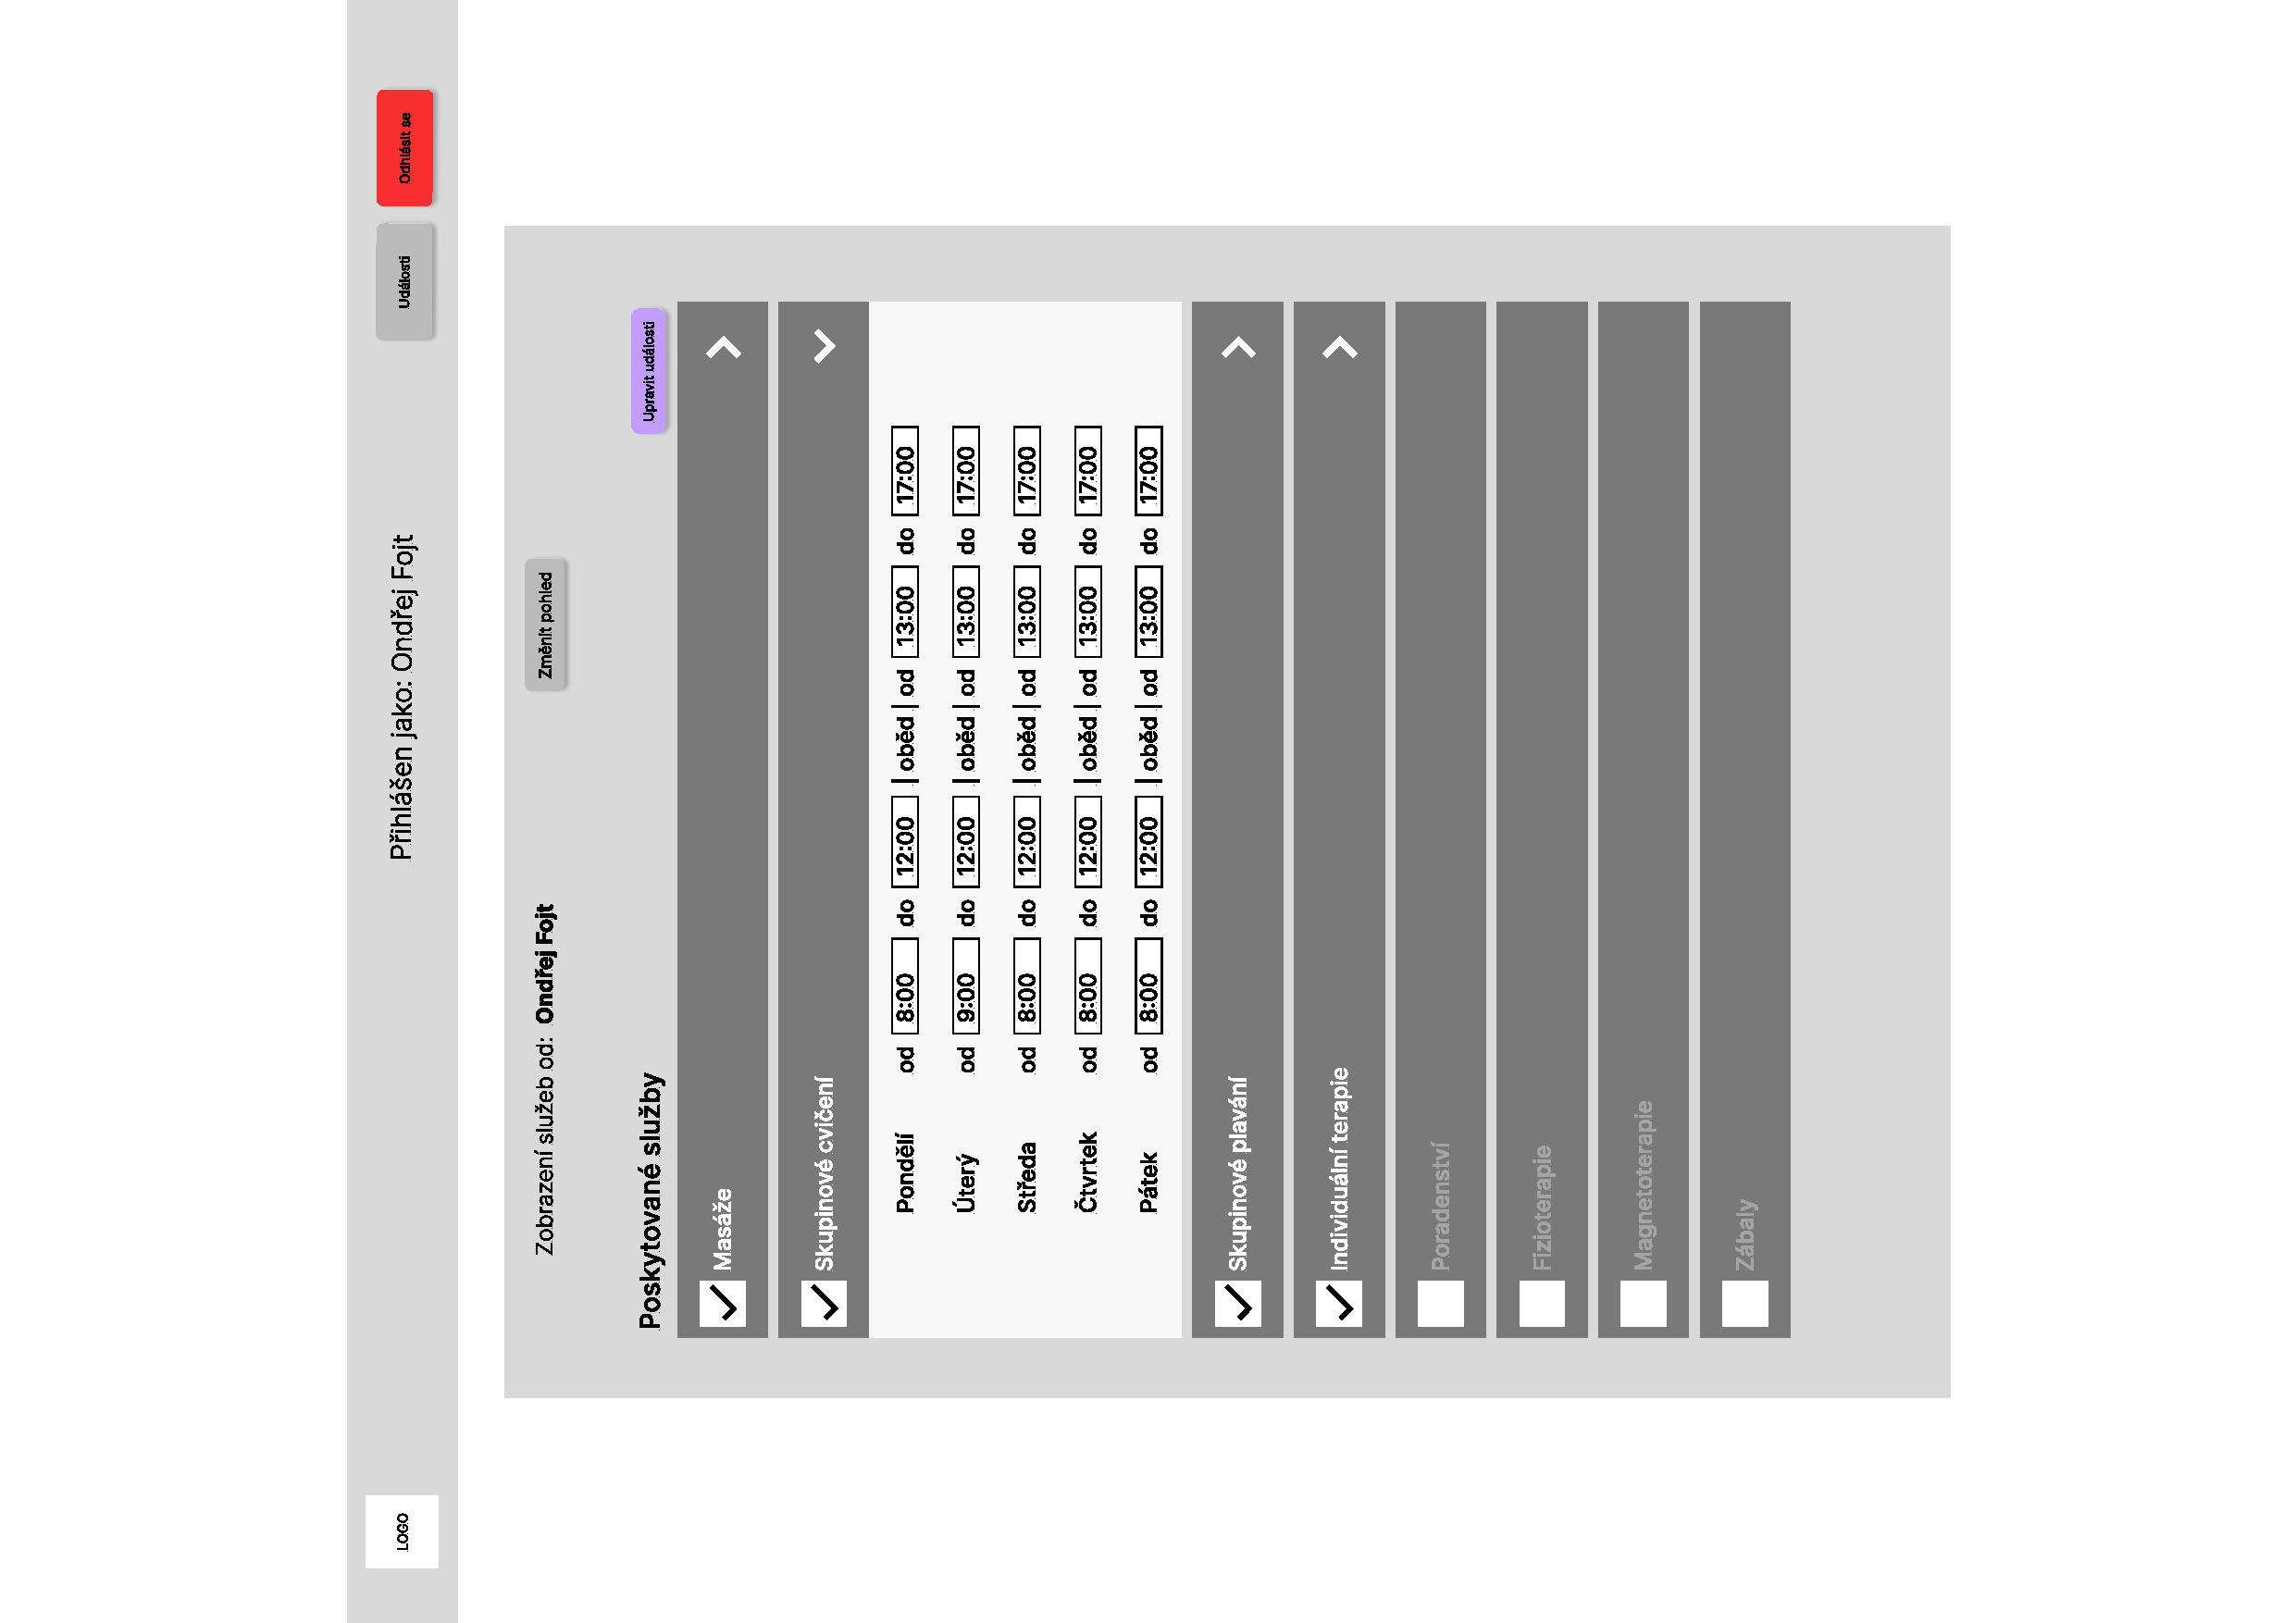
\includegraphics[angle=270, origin=c, width = \textwidth, trim=180 0 250 0, clip]{doc/latex/fig/ondra/figma3.pdf}
    \caption{Poskytované služby daného zaměstnance}
    \label{fig:Ondra_figma_services}
\end{figure}

\newpage

\subsubsection*{Testování makety}

Testována maketa pro zaměstnance výše a také pro přihlašování klientů od Vlada.
Testy byly provedeny na 3 osobách se zkušenosti z přihlašování na rehabilitace.
Testy spočívaly ve schopnosti orientace v systému a určování funkčnosti jednotlivých prvků.

Poznatky k přihlašování klientů:
\begin{itemize}
    \item Starší osoba může mít strach vkládat někde e-mail\\ pro přihlášení/registraci, kvůli reklamnímu spamu.
    \item Není jasný čas kdy se lze telefonicky spojit přímo se zaměstnancem, pokud by to bylo potřeba?\\ Někdy stačí přesměrovat hovor k vrátnici/sekretariátu.
    \item Některé osoby na rehabilitace přihlašuje například sestřička od doktora. Jak to máme z uživatelského hlediska vyřešené?
    \item Chybí cena za službu, popis dané služby a přehled přihlášky před potvrzením(ten je teoreticky odeslán v e-mailu, kde lze přihlášku zrušit... ale e-mail není 100\% spolehlivý)
\end{itemize}
Poznatky k rozhraní pro zaměstnance:
\begin{itemize}
    \item Každý se shodl, že nejbližší události by měli ukazovat pouze jeden den a že je potřeba zavést přepínání k tomuto poli mezi dny.
    \item Služby a organizační záležitosti firmy by potřeby barevné odlišení, které by nekolidovalo s odlišením nejbližší události.
    \item Nejde vyhledávat klienty.
    \item Pokud by se zobrazil kontakt na klienta tak by se hodilo vypsat, jejich termíny návštěv.
    \item Prvek \emph{Zobrazení událostí od} je buďto přehlížen nebo mu není věnována větší pozornost, především při prvním použití.
    \item Zajímavá otázka na back-end: Jakým způsobem se přidělí přihlášky zaměstnancům? Aby jeden neměl pořád přeplněno, protože má příjmení dříve v abecedě...
\end{itemize}

% README
% Pictures !!! include your own !!!
% When loading images, load zour images into fig. directory
% Then include them here and dont forget to fill capution and label please :)
%\begin{figure}[h]
%    \centering
%    \includegraphics[width = \textwidth]{doc/latex/fig/"your_image"}
%    \caption{"your_caption"}
%    \label{fig:"your_image_label"}
%\end{figure}

\subsection*{Provedené změny návrhu}

Zaměstnanec byl rozdělen na administrativního pracovníka, tedy zaměstnance, který vidí statistiky a obsazenosti služeb/procedur a zaměstnanců
a fyzioterapeuta, který je odpovědný za jednotlivé procedury.
Administrativní pracovník by měl mít také možnost přidávat a odebírat registrace pacientů na procedury.
Fyzioterapeut by měl moci potvrzovat příchod pacienta na registrace a vystavení zprávy o provedení zákroku.

Stránky pro tyto uživatele byly rozděleny členům týmu takto:
\begin{itemize}
    \item Ondřej Fojt - Administrativní pracovník
    \item Vít Hrbáček - Fyzioterapeut
\end{itemize}

\newpage
